
\chapter{DISCUSSÃO DOS RESULTADOS} 

\par Neste capitulo serão apresentados e discutidos os resultados obtidos por esta pesquisa e desenvolvimento do \textit{software}, apresentando os seus pontos positivos e negativos.

\par Inicialmente foram utilizadas as tecnologias Java, Primefaces e JSF para desenvolver este trabalho, no entanto, viu-se a necessidade de alterar algumas destas tecnologias, visando agilizar o processo de desenvolvimento. Desta forma, passou-se a utilizar HTML, CSS, Javascript em conjunto com o \textit{framework} Angular JS.

\par A mudança de tecnologias trouxe como benefício o desacoplamento das partes cliente (\textit{front-end}) e servidor (\textit{back end}), não sendo mais necessário recompilar, construir e publicar a aplicação no servidor \textit{web}, como era feito até então a cada alteração.

\par Após esta mudança, notou-se que a forma como o banco de dados era acessado poderia ser ajustada, a fim de seguir a mesma ideia proposta pela troca de tecnologias já mencionadas, uma vez que o banco de dados Neo4j permite duas maneiras de conexão, sendo elas: \textit{embedded} e por meio da API REST.(XXXXX).Desta forma, passou-se a utilizar a API REST ao invés da forma \textit{embedded}, utilizada até então.

\par Posterior a estas mudanças, deu-se continuidade no desenvolvimento da aplicação, onde os seus principais resultados da são apresentados a seguir.


\section{Buscar Serviços}

\par Uma das funcionalidades implementadas no desenvolvimento foi a busca por serviços. Esta busca permite que o usuário encontre profissionais que desempenham a função específica procurada por ele. Para realizar esta busca, foi preciso escrever uma consulta que leva em conta três níveis de análise, sendo elas, a busca pelo profissional que desempenha o trabalho dentro da rede de parceiros, dentro da empresa onde o usuário trabalha e por último, dentro da cidade onde ele vive. A ideia é apresentar um possível prestador de serviços que já tenha sido avaliado por alguém em comum ao usuário, uma vez que desta forma, há uma confiança maior em relação ao profissional que está sendo contratado. 

\par Para escrever esta consulta foi utilizada a tecnologia \textit{Cypher}, que é uma linguagem específica para o banco Neo4j \cite{neo4j_team_manual}. A Figura~\ref{fig:consulta_busca} apresenta à \textit{query} utilizada para realizar a busca.

\begin{figure}[h!]
	\centerline{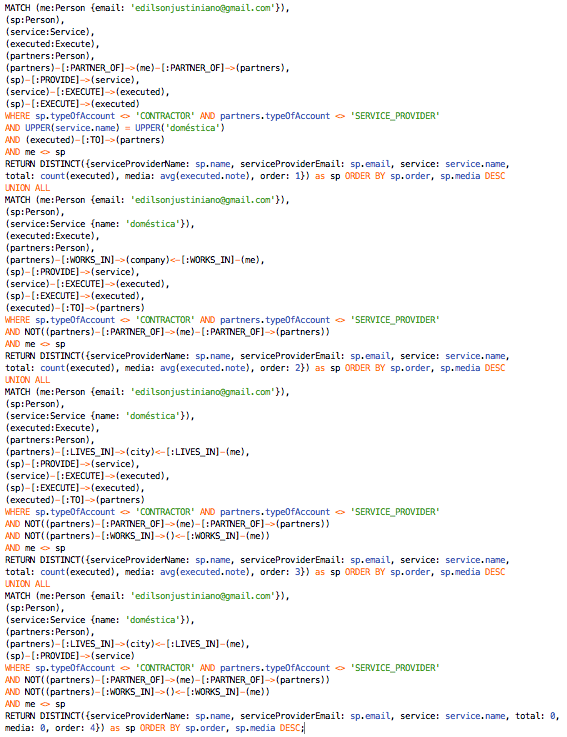
\includegraphics[scale=0.7]{./imagens/consulta-busca-domestica.png}}
	\caption[\textit{Query} para buscar serviços.]
	{\textit{Query} para buscar serviços \textbf{Fonte:} Elaborado pelos autores.}
	\label{fig:consulta_busca}
\end{figure}



\par A Figura~\ref{fig:busca_domestica_edilson} demonstra a página apresentada ao usuário após buscar o serviço solicitado. No exemplo, é apresentado o resultado ao se realizar uma busca por um profissional que desempenhe o serviço de faxineira.

\begin{figure}[h!]
	\centerline{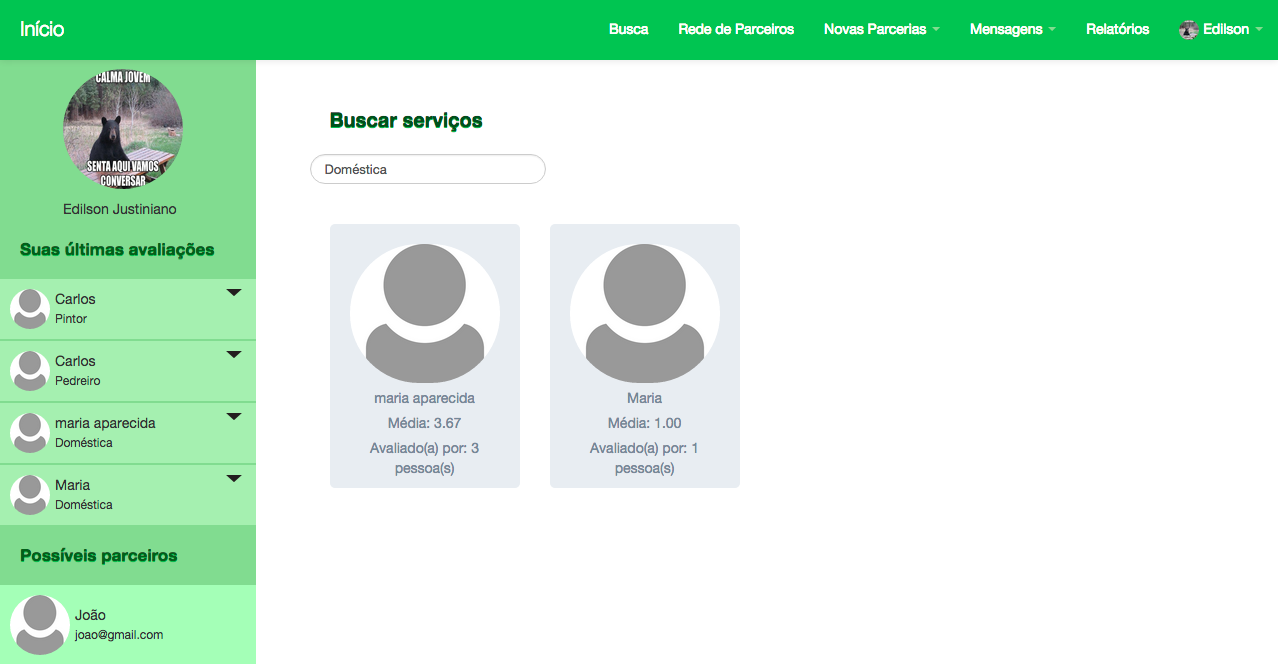
\includegraphics[scale=0.4]{./imagens/busca-domestica-edilson.png}}
	\caption[\textit Página resultante da busca por doméstica.]
	{\textit Página resultante da busca por doméstica \textbf{Fonte:} Elaborado pelos autores.}
	\label{fig:busca_domestica_edilson}
\end{figure}

\newpage

\section{Buscar novos parceiros}